\documentclass[10pt]{article}
\usepackage{tmlr}
\usepackage{microtype}
\usepackage{amsmath,amssymb}
\usepackage{booktabs}
\usepackage{array}
\usepackage{multirow}
\usepackage{longtable}
\usepackage{graphicx}
\usepackage{xspace}
\usepackage{enumitem}
\usepackage{hyperref}
\usepackage{url}

\newcommand{\method}{\textsc{TrajUQ}\xspace}
\newcommand{\tbd}{\textsc{TBD}}
\newcommand{\calp}{\widehat{p}_{\mathrm{err}}}
\newcommand{\cmark}{\checkmark}
% PRE-RESULTS FALLBACK.
% This file is replaced by scripts/render_results_tex.py after the frozen
% primary/RQ1, feature-ablation, repeated-sampling, and adaptive artifacts pass.
\newcommand{\PrimaryDecisionAUROC}{\tbd}
\newcommand{\PrimaryDecisionAUPRC}{\tbd}
\newcommand{\PrimaryDecisionBrier}{\tbd}
\newcommand{\PrimaryDecisionECE}{\tbd}
\newcommand{\PrimaryDecisionAURC}{\tbd}
\newcommand{\PrimaryTrajAUROC}{\tbd}
\newcommand{\PrimaryTrajAUPRC}{\tbd}
\newcommand{\PrimaryTrajBrier}{\tbd}
\newcommand{\PrimaryTrajECE}{\tbd}
\newcommand{\PrimaryTrajAURC}{\tbd}

\newcommand{\RepeatedAUROC}{\tbd}
\newcommand{\RepeatedAUPRC}{\tbd}
\newcommand{\RepeatedAURC}{\tbd}
\newcommand{\RepeatedTrajAUROC}{\tbd}
\newcommand{\RepeatedTrajAUPRC}{\tbd}
\newcommand{\RepeatedTrajAURC}{\tbd}
\newcommand{\RepeatedAuxWallTime}{\tbd}

\newcommand{\AblationDistributionAUROCDelta}{\tbd}
\newcommand{\AblationDistributionAUROCLow}{\tbd}
\newcommand{\AblationDistributionAUROCHigh}{\tbd}
\newcommand{\AblationDistributionAUPRCDelta}{\tbd}
\newcommand{\AblationDistributionAURCDelta}{\tbd}
\newcommand{\AblationStabilityAUROCDelta}{\tbd}
\newcommand{\AblationStabilityAUROCLow}{\tbd}
\newcommand{\AblationStabilityAUROCHigh}{\tbd}
\newcommand{\AblationStabilityAUPRCDelta}{\tbd}
\newcommand{\AblationStabilityAURCDelta}{\tbd}
\newcommand{\AblationPersistenceAUROCDelta}{\tbd}
\newcommand{\AblationPersistenceAUROCLow}{\tbd}
\newcommand{\AblationPersistenceAUROCHigh}{\tbd}
\newcommand{\AblationPersistenceAUPRCDelta}{\tbd}
\newcommand{\AblationPersistenceAURCDelta}{\tbd}
\newcommand{\AblationFullAUROCDelta}{\tbd}
\newcommand{\AblationFullAUROCLow}{\tbd}
\newcommand{\AblationFullAUROCHigh}{\tbd}
\newcommand{\AblationFullAUPRCDelta}{\tbd}
\newcommand{\AblationFullAURCDelta}{\tbd}
\newcommand{\AblationNoJSAUROCDelta}{\tbd}
\newcommand{\AblationNoJSAUROCLow}{\tbd}
\newcommand{\AblationNoJSAUROCHigh}{\tbd}
\newcommand{\AblationNoJSAUPRCDelta}{\tbd}
\newcommand{\AblationNoJSAURCDelta}{\tbd}
\newcommand{\AblationNoRevisionsAUROCDelta}{\tbd}
\newcommand{\AblationNoRevisionsAUROCLow}{\tbd}
\newcommand{\AblationNoRevisionsAUROCHigh}{\tbd}
\newcommand{\AblationNoRevisionsAUPRCDelta}{\tbd}
\newcommand{\AblationNoRevisionsAURCDelta}{\tbd}
\newcommand{\AblationNoPersistenceAUROCDelta}{\tbd}
\newcommand{\AblationNoPersistenceAUROCLow}{\tbd}
\newcommand{\AblationNoPersistenceAUROCHigh}{\tbd}
\newcommand{\AblationNoPersistenceAUPRCDelta}{\tbd}
\newcommand{\AblationNoPersistenceAURCDelta}{\tbd}

\newcommand{\AdaptiveBaseAccuracy}{\tbd}
\newcommand{\AdaptiveBaseCost}{\tbd}
\newcommand{\AdaptiveRefinedAccuracy}{\tbd}
\newcommand{\AdaptiveRefinedCost}{\tbd}
\newcommand{\AdaptiveRandomAccuracy}{\tbd}
\newcommand{\AdaptiveRandomCost}{\tbd}
\newcommand{\AdaptiveAccuracy}{\tbd}
\newcommand{\AdaptiveCost}{\tbd}
\newcommand{\AdaptiveDeltaRandom}{\tbd}

\newcommand{\AbstractResultSentence}{Empirical results are intentionally omitted from this pre-experiment manuscript and will be populated only from traceable frozen artifacts.}
\newcommand{\ResultsResultSentence}{This manuscript is currently pre-experiment. No numerical claim is populated until it can be traced to frozen artifacts.}
\newcommand{\ConclusionResultSentence}{}
\newcommand{\PaperStateLimitationsSentence}{The current manuscript is pre-experiment and therefore makes no empirical performance claim.}

\IfFileExists{generated_rq1.tex}{% GENERATED FILE -- DO NOT TYPE RESULT VALUES BY HAND.
% Complete provenance-bound RQ1 package; downstream RQs remain pending.
% source primary: results/primary_analysis/macro_primary.json sha256=de0044ffd8ec59de9137f9fcd023b8b6f8fcebc96668c9e49a4e618833b95f20
% source claim_gate: results/primary_analysis/rq1_claim_gate.json sha256=d1f5abc4c1a9451ebd44faec80d107747878f7acd8b4074ac1c21d5695a5e381
% source ablation: results/primary_analysis/macro_feature_ablation.json sha256=041c29b707a191f1ce05267d2a55d2dfe10cfc8e7df3d81b6b428bf1afacf99a
% source prior_signals: results/primary_analysis/macro_prior_signal_diagnostics.json sha256=b63a404e22e34d4c0f2bb6b2a4cf96ee6696583a8ab3c82cc0198a92e95aec02
% source calibration_sensitivity: results/primary_analysis/macro_calibration_sensitivity.json sha256=319d69238621a2b4e62ddcbb6475e5fece264b5ef04fef3b4c4469b6fb204100
% source primary_config: configs/experiments/primary.yaml sha256=d859e4da6b9c2c195f049559b8368d691c33e51ad0d411d12caa6ecaaa205788
\providecommand{\PrimaryDecisionAUROC}{}
\renewcommand{\PrimaryDecisionAUROC}{0.574}
\providecommand{\PrimaryTrajAUROC}{}
\renewcommand{\PrimaryTrajAUROC}{0.605}
\providecommand{\PrimaryDeltaAUROC}{}
\renewcommand{\PrimaryDeltaAUROC}{+0.031}
\providecommand{\PrimaryDeltaAUROCLow}{}
\renewcommand{\PrimaryDeltaAUROCLow}{+0.010}
\providecommand{\PrimaryDeltaAUROCHigh}{}
\renewcommand{\PrimaryDeltaAUROCHigh}{+0.050}
\providecommand{\PrimaryDecisionAUPRC}{}
\renewcommand{\PrimaryDecisionAUPRC}{0.664}
\providecommand{\PrimaryTrajAUPRC}{}
\renewcommand{\PrimaryTrajAUPRC}{0.685}
\providecommand{\PrimaryDeltaAUPRC}{}
\renewcommand{\PrimaryDeltaAUPRC}{+0.021}
\providecommand{\PrimaryDeltaAUPRCLow}{}
\renewcommand{\PrimaryDeltaAUPRCLow}{+0.009}
\providecommand{\PrimaryDeltaAUPRCHigh}{}
\renewcommand{\PrimaryDeltaAUPRCHigh}{+0.032}
\providecommand{\PrimaryDecisionBrier}{}
\renewcommand{\PrimaryDecisionBrier}{0.189}
\providecommand{\PrimaryTrajBrier}{}
\renewcommand{\PrimaryTrajBrier}{0.188}
\providecommand{\PrimaryDeltaBrier}{}
\renewcommand{\PrimaryDeltaBrier}{+0.001}
\providecommand{\PrimaryDeltaBrierLow}{}
\renewcommand{\PrimaryDeltaBrierLow}{-0.001}
\providecommand{\PrimaryDeltaBrierHigh}{}
\renewcommand{\PrimaryDeltaBrierHigh}{+0.004}
\providecommand{\PrimaryDecisionNLL}{}
\renewcommand{\PrimaryDecisionNLL}{0.562}
\providecommand{\PrimaryTrajNLL}{}
\renewcommand{\PrimaryTrajNLL}{0.568}
\providecommand{\PrimaryDeltaNLL}{}
\renewcommand{\PrimaryDeltaNLL}{-0.006}
\providecommand{\PrimaryDeltaNLLLow}{}
\renewcommand{\PrimaryDeltaNLLLow}{-0.018}
\providecommand{\PrimaryDeltaNLLHigh}{}
\renewcommand{\PrimaryDeltaNLLHigh}{+0.004}
\providecommand{\PrimaryDecisionECE}{}
\renewcommand{\PrimaryDecisionECE}{0.062}
\providecommand{\PrimaryTrajECE}{}
\renewcommand{\PrimaryTrajECE}{0.078}
\providecommand{\PrimaryDeltaECE}{}
\renewcommand{\PrimaryDeltaECE}{-0.016}
\providecommand{\PrimaryDeltaECELow}{}
\renewcommand{\PrimaryDeltaECELow}{-0.030}
\providecommand{\PrimaryDeltaECEHigh}{}
\renewcommand{\PrimaryDeltaECEHigh}{-0.012}
\providecommand{\PrimaryDecisionAURC}{}
\renewcommand{\PrimaryDecisionAURC}{0.562}
\providecommand{\PrimaryTrajAURC}{}
\renewcommand{\PrimaryTrajAURC}{0.529}
\providecommand{\PrimaryDeltaAURC}{}
\renewcommand{\PrimaryDeltaAURC}{+0.032}
\providecommand{\PrimaryDeltaAURCLow}{}
\renewcommand{\PrimaryDeltaAURCLow}{+0.021}
\providecommand{\PrimaryDeltaAURCHigh}{}
\renewcommand{\PrimaryDeltaAURCHigh}{+0.044}
\providecommand{\AblationDistributionAUROCDelta}{}
\renewcommand{\AblationDistributionAUROCDelta}{+0.022}
\providecommand{\AblationDistributionAUROCLow}{}
\renewcommand{\AblationDistributionAUROCLow}{+0.007}
\providecommand{\AblationDistributionAUROCHigh}{}
\renewcommand{\AblationDistributionAUROCHigh}{+0.036}
\providecommand{\AblationDistributionAUPRCDelta}{}
\renewcommand{\AblationDistributionAUPRCDelta}{+0.019}
\providecommand{\AblationDistributionAURCDelta}{}
\renewcommand{\AblationDistributionAURCDelta}{+0.019}
\providecommand{\AblationStabilityAUROCDelta}{}
\renewcommand{\AblationStabilityAUROCDelta}{+0.018}
\providecommand{\AblationStabilityAUROCLow}{}
\renewcommand{\AblationStabilityAUROCLow}{-0.003}
\providecommand{\AblationStabilityAUROCHigh}{}
\renewcommand{\AblationStabilityAUROCHigh}{+0.037}
\providecommand{\AblationStabilityAUPRCDelta}{}
\renewcommand{\AblationStabilityAUPRCDelta}{+0.011}
\providecommand{\AblationStabilityAURCDelta}{}
\renewcommand{\AblationStabilityAURCDelta}{+0.021}
\providecommand{\AblationPersistenceAUROCDelta}{}
\renewcommand{\AblationPersistenceAUROCDelta}{+0.002}
\providecommand{\AblationPersistenceAUROCLow}{}
\renewcommand{\AblationPersistenceAUROCLow}{-0.006}
\providecommand{\AblationPersistenceAUROCHigh}{}
\renewcommand{\AblationPersistenceAUROCHigh}{+0.009}
\providecommand{\AblationPersistenceAUPRCDelta}{}
\renewcommand{\AblationPersistenceAUPRCDelta}{-0.001}
\providecommand{\AblationPersistenceAURCDelta}{}
\renewcommand{\AblationPersistenceAURCDelta}{+0.002}
\providecommand{\AblationFullAUROCDelta}{}
\renewcommand{\AblationFullAUROCDelta}{+0.031}
\providecommand{\AblationFullAUROCLow}{}
\renewcommand{\AblationFullAUROCLow}{+0.010}
\providecommand{\AblationFullAUROCHigh}{}
\renewcommand{\AblationFullAUROCHigh}{+0.050}
\providecommand{\AblationFullAUPRCDelta}{}
\renewcommand{\AblationFullAUPRCDelta}{+0.021}
\providecommand{\AblationFullAURCDelta}{}
\renewcommand{\AblationFullAURCDelta}{+0.032}
\providecommand{\AblationNoJSAUROCDelta}{}
\renewcommand{\AblationNoJSAUROCDelta}{+0.026}
\providecommand{\AblationNoJSAUROCLow}{}
\renewcommand{\AblationNoJSAUROCLow}{+0.009}
\providecommand{\AblationNoJSAUROCHigh}{}
\renewcommand{\AblationNoJSAUROCHigh}{+0.042}
\providecommand{\AblationNoJSAUPRCDelta}{}
\renewcommand{\AblationNoJSAUPRCDelta}{+0.019}
\providecommand{\AblationNoJSAURCDelta}{}
\renewcommand{\AblationNoJSAURCDelta}{+0.024}
\providecommand{\AblationNoRevisionsAUROCDelta}{}
\renewcommand{\AblationNoRevisionsAUROCDelta}{+0.028}
\providecommand{\AblationNoRevisionsAUROCLow}{}
\renewcommand{\AblationNoRevisionsAUROCLow}{+0.008}
\providecommand{\AblationNoRevisionsAUROCHigh}{}
\renewcommand{\AblationNoRevisionsAUROCHigh}{+0.047}
\providecommand{\AblationNoRevisionsAUPRCDelta}{}
\renewcommand{\AblationNoRevisionsAUPRCDelta}{+0.019}
\providecommand{\AblationNoRevisionsAURCDelta}{}
\renewcommand{\AblationNoRevisionsAURCDelta}{+0.030}
\providecommand{\AblationNoPersistenceAUROCDelta}{}
\renewcommand{\AblationNoPersistenceAUROCDelta}{+0.032}
\providecommand{\AblationNoPersistenceAUROCLow}{}
\renewcommand{\AblationNoPersistenceAUROCLow}{+0.012}
\providecommand{\AblationNoPersistenceAUROCHigh}{}
\renewcommand{\AblationNoPersistenceAUROCHigh}{+0.050}
\providecommand{\AblationNoPersistenceAUPRCDelta}{}
\renewcommand{\AblationNoPersistenceAUPRCDelta}{+0.023}
\providecommand{\AblationNoPersistenceAURCDelta}{}
\renewcommand{\AblationNoPersistenceAURCDelta}{+0.034}
\providecommand{\PriorEntropyAUROC}{}
\renewcommand{\PriorEntropyAUROC}{0.567}
\providecommand{\PriorEntropyTrajAUROC}{}
\renewcommand{\PriorEntropyTrajAUROC}{0.605}
\providecommand{\PriorEntropyAUROCDelta}{}
\renewcommand{\PriorEntropyAUROCDelta}{+0.038}
\providecommand{\PriorEntropyAUROCLow}{}
\renewcommand{\PriorEntropyAUROCLow}{+0.018}
\providecommand{\PriorEntropyAUROCHigh}{}
\renewcommand{\PriorEntropyAUROCHigh}{+0.056}
\providecommand{\PriorEntropyAUPRCDelta}{}
\renewcommand{\PriorEntropyAUPRCDelta}{+0.022}
\providecommand{\PriorEntropyAURCDelta}{}
\renewcommand{\PriorEntropyAURCDelta}{+0.041}
\providecommand{\PriorFlipRateAUROC}{}
\renewcommand{\PriorFlipRateAUROC}{0.544}
\providecommand{\PriorFlipRateTrajAUROC}{}
\renewcommand{\PriorFlipRateTrajAUROC}{0.605}
\providecommand{\PriorFlipRateAUROCDelta}{}
\renewcommand{\PriorFlipRateAUROCDelta}{+0.061}
\providecommand{\PriorFlipRateAUROCLow}{}
\renewcommand{\PriorFlipRateAUROCLow}{+0.042}
\providecommand{\PriorFlipRateAUROCHigh}{}
\renewcommand{\PriorFlipRateAUROCHigh}{+0.081}
\providecommand{\PriorFlipRateAUPRCDelta}{}
\renewcommand{\PriorFlipRateAUPRCDelta}{+0.040}
\providecommand{\PriorFlipRateAURCDelta}{}
\renewcommand{\PriorFlipRateAURCDelta}{+0.052}
\providecommand{\CalibrationEligibleCells}{}
\renewcommand{\CalibrationEligibleCells}{6}
\providecommand{\CalibrationSkippedCells}{}
\renewcommand{\CalibrationSkippedCells}{12}
\providecommand{\CalibrationDecisionBrierLogistic}{}
\renewcommand{\CalibrationDecisionBrierLogistic}{0.181}
\providecommand{\CalibrationDecisionBrierIsotonic}{}
\renewcommand{\CalibrationDecisionBrierIsotonic}{0.181}
\providecommand{\CalibrationDecisionBrierDelta}{}
\renewcommand{\CalibrationDecisionBrierDelta}{+0.000}
\providecommand{\CalibrationDecisionNLLLogistic}{}
\renewcommand{\CalibrationDecisionNLLLogistic}{0.544}
\providecommand{\CalibrationDecisionNLLIsotonic}{}
\renewcommand{\CalibrationDecisionNLLIsotonic}{0.576}
\providecommand{\CalibrationDecisionNLLDelta}{}
\renewcommand{\CalibrationDecisionNLLDelta}{-0.032}
\providecommand{\CalibrationDecisionECELogistic}{}
\renewcommand{\CalibrationDecisionECELogistic}{0.056}
\providecommand{\CalibrationDecisionECEIsotonic}{}
\renewcommand{\CalibrationDecisionECEIsotonic}{0.049}
\providecommand{\CalibrationDecisionECEDelta}{}
\renewcommand{\CalibrationDecisionECEDelta}{+0.007}
\providecommand{\CalibrationDecisionAURCLogistic}{}
\renewcommand{\CalibrationDecisionAURCLogistic}{0.364}
\providecommand{\CalibrationDecisionAURCIsotonic}{}
\renewcommand{\CalibrationDecisionAURCIsotonic}{0.356}
\providecommand{\CalibrationDecisionAURCDelta}{}
\renewcommand{\CalibrationDecisionAURCDelta}{+0.008}
\providecommand{\CalibrationTrajBrierLogistic}{}
\renewcommand{\CalibrationTrajBrierLogistic}{0.174}
\providecommand{\CalibrationTrajBrierIsotonic}{}
\renewcommand{\CalibrationTrajBrierIsotonic}{0.175}
\providecommand{\CalibrationTrajBrierDelta}{}
\renewcommand{\CalibrationTrajBrierDelta}{-0.001}
\providecommand{\CalibrationTrajNLLLogistic}{}
\renewcommand{\CalibrationTrajNLLLogistic}{0.531}
\providecommand{\CalibrationTrajNLLIsotonic}{}
\renewcommand{\CalibrationTrajNLLIsotonic}{0.540}
\providecommand{\CalibrationTrajNLLDelta}{}
\renewcommand{\CalibrationTrajNLLDelta}{-0.009}
\providecommand{\CalibrationTrajECELogistic}{}
\renewcommand{\CalibrationTrajECELogistic}{0.052}
\providecommand{\CalibrationTrajECEIsotonic}{}
\renewcommand{\CalibrationTrajECEIsotonic}{0.040}
\providecommand{\CalibrationTrajECEDelta}{}
\renewcommand{\CalibrationTrajECEDelta}{+0.011}
\providecommand{\CalibrationTrajAURCLogistic}{}
\renewcommand{\CalibrationTrajAURCLogistic}{0.328}
\providecommand{\CalibrationTrajAURCIsotonic}{}
\renewcommand{\CalibrationTrajAURCIsotonic}{0.332}
\providecommand{\CalibrationTrajAURCDelta}{}
\renewcommand{\CalibrationTrajAURCDelta}{-0.004}
\providecommand{\AbstractResultSentence}{}
\renewcommand{\AbstractResultSentence}{Across the frozen 18-cell matrix, trajectory features improve macro AUROC over decision-time entropy by +0.031 (95\% CI [+0.010, +0.050]), with positive point improvement in 2/3 model families.}
\providecommand{\ResultsResultSentence}{}
\renewcommand{\ResultsResultSentence}{The pre-registered RQ1 positive-claim gate is met: equal-cell macro AUROC improves by +0.031 (95\% CI [+0.010, +0.050]) and 2/3 model families improve. The gain is heterogeneous: LLaDA and Dream improve while SDAR does not, and ECE worsens despite gains in discrimination and selective risk.}
\providecommand{\ConclusionResultSentence}{}
\renewcommand{\ConclusionResultSentence}{The frozen primary analysis yields a macro AUROC improvement of +0.031 over decision-time entropy and satisfies the pre-registered RQ1 gate, with model-family and calibration heterogeneity retained as first-class findings.}
\providecommand{\PaperStateLimitationsSentence}{}
\renewcommand{\PaperStateLimitationsSentence}{RQ1 is complete and provenance-bound; RQ2--RQ5 claims remain provisional until their respective frozen registries pass final validation.}
\providecommand{\DetailedPrimaryTable}{}
\renewcommand{\DetailedPrimaryTable}{\section{Per-Cell Held-Out Results}
\label{sec:per-cell-results}
\begin{table*}[t]
\centering
\scriptsize
\setlength{\tabcolsep}{2.8pt}
\renewcommand{\arraystretch}{1.08}
\begin{tabular*}{\textwidth}{@{\extracolsep{\fill}}llrrrrrrrr@{}}
\toprule
Model & Dataset & $n$ & Err. & \multicolumn{3}{c}{AUROC $\uparrow$} & \multicolumn{3}{c}{AURC $\downarrow$}\\
\cmidrule(lr){5-7}\cmidrule(lr){8-10}
 & & & (\%) & Decision & \method & $\Delta$ & Decision & \method & $\Delta$\\
\midrule
LLaDA & GSM8K & 500 & 54.4\% & 0.730 & 0.764 & +0.034 & 0.416 & 0.345 & +0.071\\
LLaDA & MATH-500 & 347 & 77.5\% & 0.626 & 0.696 & +0.070 & 0.727 & 0.630 & +0.097\\
LLaDA & GPQA-Diamond & 142 & 71.1\% & 0.523 & 0.460 & -0.064 & 0.691 & 0.718 & -0.028\\
LLaDA & ARC-Challenge & 500 & 13.6\% & 0.544 & 0.592 & +0.048 & 0.136 & 0.104 & +0.032\\
LLaDA & MMLU-Pro & 500 & 62.6\% & 0.523 & 0.593 & +0.070 & 0.630 & 0.548 & +0.082\\
LLaDA & TruthfulQA & 572 & 48.3\% & 0.469 & 0.674 & +0.204 & 0.510 & 0.362 & +0.148\\
\addlinespace[1pt]
SDAR & GSM8K & 500 & 63.4\% & 0.695 & 0.709 & +0.014 & 0.523 & 0.481 & +0.042\\
SDAR & MATH-500 & 347 & 95.1\% & 0.612 & 0.467 & -0.145 & 0.933 & 0.955 & -0.022\\
SDAR & GPQA-Diamond & 142 & 80.3\% & 0.500 & 0.519 & +0.019 & 0.820 & 0.805 & +0.015\\
SDAR & ARC-Challenge & 500 & 68.4\% & 0.535 & 0.588 & +0.053 & 0.677 & 0.623 & +0.054\\
SDAR & MMLU-Pro & 500 & 87.2\% & 0.537 & 0.559 & +0.021 & 0.855 & 0.857 & -0.002\\
SDAR & TruthfulQA & 572 & 39.5\% & 0.595 & 0.559 & -0.036 & 0.317 & 0.342 & -0.024\\
\addlinespace[1pt]
Dream & GSM8K & 500 & 50.2\% & 0.739 & 0.769 & +0.031 & 0.310 & 0.287 & +0.023\\
Dream & MATH-500 & 347 & 77.8\% & 0.584 & 0.677 & +0.093 & 0.669 & 0.657 & +0.012\\
Dream & GPQA-Diamond & 142 & 73.9\% & 0.574 & 0.560 & -0.014 & 0.676 & 0.691 & -0.015\\
Dream & ARC-Challenge & 500 & 13.4\% & 0.557 & 0.558 & +0.001 & 0.122 & 0.125 & -0.003\\
Dream & MMLU-Pro & 500 & 56.2\% & 0.485 & 0.481 & -0.004 & 0.570 & 0.568 & +0.002\\
Dream & TruthfulQA & 572 & 54.4\% & 0.498 & 0.663 & +0.165 & 0.528 & 0.429 & +0.100\\
\bottomrule
\end{tabular*}
\caption{Per-cell held-out discrimination and selective-risk results for the complete frozen $3\times6$ matrix. $\Delta$ is oriented so positive values favor \method: candidate minus baseline for AUROC and baseline minus candidate for lower-is-better AURC. The table is generated directly from the same provenance-bound primary aggregate used by the macro analysis.}
\label{tab:per-cell-primary}
\end{table*}}
\newcommand{\RQOneSummaryTable}{\begin{table*}[t]
\centering
\small
\begin{tabular}{lrrr}
\toprule
Metric & Decision entropy & \method & Oriented $\Delta$ (95\% CI)\\
\midrule
AUROC $\uparrow$ & 0.574 & 0.605 & +0.031 [+0.010, +0.050]\\
AUPRC $\uparrow$ & 0.664 & 0.685 & +0.021 [+0.009, +0.032]\\
Brier $\downarrow$ & 0.189 & 0.188 & +0.001 [-0.001, +0.004]\\
NLL $\downarrow$ & 0.562 & 0.568 & -0.006 [-0.018, +0.004]\\
ECE$_{15}$ $\downarrow$ & 0.062 & 0.078 & -0.016 [-0.030, -0.012]\\
AURC $\downarrow$ & 0.562 & 0.529 & +0.032 [+0.021, +0.044]\\
\bottomrule
\end{tabular}
\caption{Complete frozen RQ1 equal-cell macro results over 18 model--dataset cells. Improvements are oriented so positive values favor \method; lower-is-better metrics therefore use baseline minus candidate. Confidence intervals are paired, class-stratified within cell and macro-averaged across cells.}
\label{tab:rq1-complete}
\end{table*}}
}{}
% PRE-RESULTS RQ5 FALLBACK.
% The Overleaf packager replaces this file only from a validated generated
% registry manifest. Unfinished cells remain explicitly pending.
\newcommand{\RQFiveValidatedResponses}{0}
\newcommand{\RQFiveExpectedResponses}{58260}
\newcommand{\RQFiveTables}{%
\begin{table*}[t]\centering\small
\begin{tabular}{llrrl}\toprule
Model & Dataset & Validated requests & Accuracy & State \\ \midrule
DeepSeek-V3.2 & all frozen datasets & 0/19420 & -- & pending \\
GLM-5.1 & all frozen datasets & 0/19420 & -- & pending \\
Kimi-K2.6 & all frozen datasets & 0/19420 & -- & pending \\
\bottomrule\end{tabular}
\caption{RQ5 black-box execution registry. Final empirical values are generated only from the complete validated artifact registry.}
\label{tab:rq5-partial-registry}\end{table*}}

\IfFileExists{generated_synthesis.tex}{% AUTO-GENERATED from provenance-bound synthesis artifacts; do not edit.

% SYNTHESIS STATE: PROVISIONAL

\newcommand{\CrossModelSynthesisState}{PROVISIONAL}

\newcommand{\CrossModelSynthesisTable}{%
\begin{table*}[t]
\centering
\small
\setlength{\tabcolsep}{4.5pt}
\begin{tabular}{lllrrr}
\toprule
System & Observability regime & Principal signal & AUROC $\uparrow$ & $\Delta$ AUROC$^\dagger$ $\uparrow$ & AURC $\downarrow$ \\
\midrule
Dream-v0-Instruct-7B & Diffusion trajectory & native trajectory & 0.618 & 0.045 & 0.459 \\
LLaDA-MoE-7B-A1B-Instruct & Diffusion trajectory & native trajectory & 0.630 & 0.060 & 0.451 \\
SDAR-1.7B-Chat & Diffusion trajectory & native trajectory & 0.567 & -0.012 & 0.677 \\
\addlinespace[2pt]
Llama-3.1-8B-Instruct & Autoregressive trace & AR trace & \textit{pending} & \textit{pending} & \textit{pending} \\
\addlinespace[2pt]
DeepSeek-V3.2 & Black-box behavior & behavioral repeats & \textit{pending} & \textit{pending} & \textit{pending} \\
GLM-5.1 & Black-box behavior & behavioral repeats & \textit{pending} & \textit{pending} & \textit{pending} \\
Kimi-K2.6 & Black-box behavior & behavioral repeats & \textit{pending} & \textit{pending} & \textit{pending} \\
\bottomrule
\end{tabular}
\caption{What uncertainty information is observable and useful under each access regime. Values are equal-dataset-weight summaries within their registered regime; $\Delta$ AUROC compares only with the pre-registered baseline from the same regime. This is a provisional synthesis: pending entries are not estimates and support no final cross-regime claim. The table is descriptive across regimes and must not be read as a raw cross-protocol model ranking.}
\label{tab:cross-model-synthesis}
\end{table*}}

\newcommand{\CrossModelAppendixTable}{%
\begin{table*}[p]
\centering
\small
\setlength{\tabcolsep}{3.2pt}
\begin{tabular}{llrrrrrrr}
\toprule
System & Dataset & $n$ & AUROC $\uparrow$ & AUPRC $\uparrow$ & AURC $\downarrow$ & ECE$_{15}$ $\downarrow$ & Risk@50 $\downarrow$ & $\Delta$ AUROC$^\dagger$ $\uparrow$ \\
\midrule
Dream & gsm8k & 500 & 0.769 & 0.745 & 0.287 & 0.044 & 0.312 & 0.031 \\
Dream & math500 & 347 & 0.677 & 0.853 & 0.657 & 0.048 & 0.695 & 0.093 \\
Dream & gpqa\_diamond & 142 & 0.560 & 0.779 & 0.691 & 0.151 & 0.746 & -0.014 \\
Dream & arc\_challenge & 500 & 0.558 & 0.208 & 0.125 & 0.042 & 0.120 & 0.001 \\
Dream & mmlu\_pro & 500 & 0.481 & 0.558 & 0.568 & 0.110 & 0.580 & -0.004 \\
Dream & truthfulqa & 572 & 0.663 & 0.680 & 0.429 & 0.060 & 0.423 & 0.165 \\
\addlinespace[2pt]
LLaDA & gsm8k & 500 & 0.764 & 0.771 & 0.345 & 0.057 & 0.336 & 0.034 \\
LLaDA & math500 & 347 & 0.696 & 0.859 & 0.630 & 0.080 & 0.695 & 0.070 \\
LLaDA & gpqa\_diamond & 142 & 0.460 & 0.692 & 0.718 & 0.095 & 0.718 & -0.064 \\
LLaDA & arc\_challenge & 500 & 0.592 & 0.216 & 0.104 & 0.042 & 0.108 & 0.048 \\
LLaDA & mmlu\_pro & 500 & 0.593 & 0.688 & 0.548 & 0.142 & 0.568 & 0.070 \\
LLaDA & truthfulqa & 572 & 0.674 & 0.639 & 0.362 & 0.051 & 0.346 & 0.204 \\
\addlinespace[2pt]
SDAR & gsm8k & 500 & 0.709 & 0.797 & 0.481 & 0.063 & 0.476 & 0.014 \\
SDAR & math500 & 347 & 0.467 & 0.948 & 0.955 & 0.037 & 0.960 & -0.145 \\
SDAR & gpqa\_diamond & 142 & 0.519 & 0.838 & 0.805 & 0.142 & 0.803 & 0.019 \\
SDAR & arc\_challenge & 500 & 0.588 & 0.733 & 0.623 & 0.061 & 0.628 & 0.053 \\
SDAR & mmlu\_pro & 500 & 0.559 & 0.887 & 0.857 & 0.100 & 0.844 & 0.021 \\
SDAR & truthfulqa & 572 & 0.559 & 0.430 & 0.342 & 0.082 & 0.350 & -0.036 \\
\bottomrule
\end{tabular}
\caption{Diffusion-trajectory observability: complete model--dataset synthesis registry. \textit{pending} denotes a registered cell whose authoritative aggregate is not yet available; \textemdash{} denotes a genuinely unavailable or scientifically inapplicable quantity, never a measured zero. $\Delta$ values use only the appropriate within-regime baseline.}
\label{tab:cross-model-synthesis-diffusion-trajectory}
\end{table*}

\begin{table*}[p]
\centering
\small
\setlength{\tabcolsep}{3.2pt}
\begin{tabular}{llrrrrrrr}
\toprule
System & Dataset & $n$ & AUROC $\uparrow$ & AUPRC $\uparrow$ & AURC $\downarrow$ & ECE$_{15}$ $\downarrow$ & Risk@50 $\downarrow$ & $\Delta$ AUROC$^\dagger$ $\uparrow$ \\
\midrule
Llama 3.1 & gsm8k & \textit{pending} & \textit{pending} & \textit{pending} & \textit{pending} & \textit{pending} & \textit{pending} & \textit{pending} \\
Llama 3.1 & math500 & \textit{pending} & \textit{pending} & \textit{pending} & \textit{pending} & \textit{pending} & \textit{pending} & \textit{pending} \\
Llama 3.1 & gpqa\_diamond & \textit{pending} & \textit{pending} & \textit{pending} & \textit{pending} & \textit{pending} & \textit{pending} & \textit{pending} \\
Llama 3.1 & arc\_challenge & \textit{pending} & \textit{pending} & \textit{pending} & \textit{pending} & \textit{pending} & \textit{pending} & \textit{pending} \\
Llama 3.1 & mmlu\_pro & \textit{pending} & \textit{pending} & \textit{pending} & \textit{pending} & \textit{pending} & \textit{pending} & \textit{pending} \\
Llama 3.1 & truthfulqa & \textit{pending} & \textit{pending} & \textit{pending} & \textit{pending} & \textit{pending} & \textit{pending} & \textit{pending} \\
\bottomrule
\end{tabular}
\caption{Autoregressive-trace observability: complete model--dataset synthesis registry. \textit{pending} denotes a registered cell whose authoritative aggregate is not yet available; \textemdash{} denotes a genuinely unavailable or scientifically inapplicable quantity, never a measured zero. $\Delta$ values use only the appropriate within-regime baseline.}
\label{tab:cross-model-synthesis-autoregressive-trace}
\end{table*}

\begin{table*}[p]
\centering
\small
\setlength{\tabcolsep}{3.2pt}
\begin{tabular}{llrrrrrrr}
\toprule
System & Dataset & $n$ & AUROC $\uparrow$ & AUPRC $\uparrow$ & AURC $\downarrow$ & ECE$_{15}$ $\downarrow$ & Risk@50 $\downarrow$ & $\Delta$ AUROC$^\dagger$ $\uparrow$ \\
\midrule
DeepSeek & gsm8k & \textit{pending} & \textit{pending} & \textit{pending} & \textit{pending} & \textit{pending} & \textit{pending} & \textit{pending} \\
DeepSeek & math500 & \textit{pending} & \textit{pending} & \textit{pending} & \textit{pending} & \textit{pending} & \textit{pending} & \textit{pending} \\
DeepSeek & gpqa\_diamond & \textit{pending} & \textit{pending} & \textit{pending} & \textit{pending} & \textit{pending} & \textit{pending} & \textit{pending} \\
DeepSeek & arc\_challenge & \textit{pending} & \textit{pending} & \textit{pending} & \textit{pending} & \textit{pending} & \textit{pending} & \textit{pending} \\
DeepSeek & mmlu\_pro & \textit{pending} & \textit{pending} & \textit{pending} & \textit{pending} & \textit{pending} & \textit{pending} & \textit{pending} \\
DeepSeek & truthfulqa & \textit{pending} & \textit{pending} & \textit{pending} & \textit{pending} & \textit{pending} & \textit{pending} & \textit{pending} \\
\addlinespace[2pt]
GLM & gsm8k & \textit{pending} & \textit{pending} & \textit{pending} & \textit{pending} & \textit{pending} & \textit{pending} & \textit{pending} \\
GLM & math500 & \textit{pending} & \textit{pending} & \textit{pending} & \textit{pending} & \textit{pending} & \textit{pending} & \textit{pending} \\
GLM & gpqa\_diamond & \textit{pending} & \textit{pending} & \textit{pending} & \textit{pending} & \textit{pending} & \textit{pending} & \textit{pending} \\
GLM & arc\_challenge & \textit{pending} & \textit{pending} & \textit{pending} & \textit{pending} & \textit{pending} & \textit{pending} & \textit{pending} \\
GLM & mmlu\_pro & \textit{pending} & \textit{pending} & \textit{pending} & \textit{pending} & \textit{pending} & \textit{pending} & \textit{pending} \\
GLM & truthfulqa & \textit{pending} & \textit{pending} & \textit{pending} & \textit{pending} & \textit{pending} & \textit{pending} & \textit{pending} \\
\addlinespace[2pt]
Kimi & gsm8k & \textit{pending} & \textit{pending} & \textit{pending} & \textit{pending} & \textit{pending} & \textit{pending} & \textit{pending} \\
Kimi & math500 & \textit{pending} & \textit{pending} & \textit{pending} & \textit{pending} & \textit{pending} & \textit{pending} & \textit{pending} \\
Kimi & gpqa\_diamond & \textit{pending} & \textit{pending} & \textit{pending} & \textit{pending} & \textit{pending} & \textit{pending} & \textit{pending} \\
Kimi & arc\_challenge & \textit{pending} & \textit{pending} & \textit{pending} & \textit{pending} & \textit{pending} & \textit{pending} & \textit{pending} \\
Kimi & mmlu\_pro & \textit{pending} & \textit{pending} & \textit{pending} & \textit{pending} & \textit{pending} & \textit{pending} & \textit{pending} \\
Kimi & truthfulqa & \textit{pending} & \textit{pending} & \textit{pending} & \textit{pending} & \textit{pending} & \textit{pending} & \textit{pending} \\
\bottomrule
\end{tabular}
\caption{Black-box behavioral observability: complete model--dataset synthesis registry. \textit{pending} denotes a registered cell whose authoritative aggregate is not yet available; \textemdash{} denotes a genuinely unavailable or scientifically inapplicable quantity, never a measured zero. $\Delta$ values use only the appropriate within-regime baseline.}
\label{tab:cross-model-synthesis-black-box-behavior}
\end{table*}}

\newcommand{\CrossModelSignalTable}{%
\begin{table*}[p]
\centering
\small
\setlength{\tabcolsep}{3pt}
\begin{tabular}{p{2.7cm}p{5.2cm}rrrrr}
\toprule
System & Architecture/access & Parameters & Cost$^\ddagger$ & Revision & Persistence & Commitment \\
\midrule
Dream-v0-Instruct-7B & masked diffusion language model & 7.62B & \textit{pending} & yes & yes & yes \\
LLaDA-MoE-7B-A1B-Instruct & masked diffusion mixture-of-experts language model & 7.36B & \textit{pending} & yes & yes & yes \\
SDAR-1.7B-Chat & blockwise diffusion language model & 2.03B & \textit{pending} & yes & yes & yes \\
Llama-3.1-8B-Instruct & autoregressive decoder-only transformer & 8.03B & \textit{pending} & \textemdash{} & \textemdash{} & \textemdash{} \\
DeepSeek-V3.2 & black-box hosted language model & \textemdash{} & \textit{pending} & \textemdash{} & \textemdash{} & \textemdash{} \\
GLM-5.1 & black-box hosted language model & \textemdash{} & \textit{pending} & \textemdash{} & \textemdash{} & \textemdash{} \\
Kimi-K2.6 & black-box hosted language model & \textemdash{} & \textit{pending} & \textemdash{} & \textemdash{} & \textemdash{} \\
\bottomrule
\end{tabular}
\caption{Structural availability of uncertainty signals. $^\ddagger$Compute/API cost is populated only from a model-bound authoritative ledger; it is never inferred from nominal rental prices. An em dash marks a signal or parameter count that is structurally inapplicable or not exposed by the access interface. It is distinct from \textit{pending}, which means that an authorized empirical aggregate has not yet passed its final registry gate.}
\label{tab:cross-model-signal-availability}
\end{table*}}
}{
  \newcommand{\CrossModelSynthesisTable}{}
  \newcommand{\CrossModelAppendixTable}{}
  \newcommand{\CrossModelSignalTable}{}
}
% PRE-ARTIFACT FALLBACK. Replaced from the compute-budget manifest by the packager.
\newcommand{\ComputeLedgerStatus}{pending}
\newcommand{\TotalPrimaryGPUHours}{0.00}
\newcommand{\TotalRQTwoThreeGPUHours}{0.00}
\newcommand{\TotalRQFourGPUHours}{0.00}
\newcommand{\TotalAuthoritativeGPUHours}{0.00}
\newcommand{\TotalDiagnosticGPUHours}{not exactly reconstructable}
\newcommand{\TotalProjectGPUHours}{not exactly reconstructable}
\newcommand{\RQFiveRequests}{0}
\newcommand{\RQFiveInputTokens}{0}
\newcommand{\RQFiveOutputTokens}{0}
\newcommand{\RQFiveCostRMB}{0.00}
\newcommand{\CurrentRentalElapsedHours}{0.0}
\newcommand{\ComputeBudgetTable}{}
\newcommand{\ComputeBudgetAppendixTable}{}


\title{When Language Models Are Unsure During Generation:\\
Trajectory-Aware Uncertainty Across Open and Black-Box Decoding}
\author{\name Anonymous Authors}

\begin{document}
\maketitle
\footnotetext{Large language models were used as general-purpose assistive tools for language editing and software support. The authors reviewed all content and take full responsibility for the ideas, claims, analyses, and reported results.}

\begin{abstract}
Diffusion language models generate text by repeatedly revising partially masked sequences, exposing a temporal signal that autoregressive confidence estimators do not observe.
We study whether this denoising trajectory can reveal answer-level failure \emph{before} benchmark correctness is known.
We introduce \method, a training-free telemetry framework with post-hoc calibration that measures uncertainty only on positions that are active and unresolved at each denoising step.
Its features combine predictive entropy and margin, consecutive-step Jensen--Shannon drift, proposal revisions, mask persistence, and commitment timing.
A held-out calibrator maps these pre-outcome signals to error probability, which supports selective generation and a two-budget adaptive-compute policy.
The primary test is deliberately nested: a trajectory-augmented predictor must improve over a strong per-token decision-time entropy baseline evaluated on the same held-out examples.
We further compare against repeated-sampling disagreement under explicit compute accounting, study three open diffusion families, and prospectively evaluate Llama-3.1-8B-Instruct as an autoregressive control on the same frozen tasks and partitions.
A separately registered black-box extension evaluates three hosted API families using only deployment-visible behavioral signals.
Together, these comparisons separate uncertainty dynamics shared by sequential generation from revision, persistence, and commitment signals specific to iterative denoising, and test what remains useful when internal probabilities are unavailable.
All model, data, feature, calibration, and statistical choices are frozen before primary test outcomes are inspected.
\AbstractResultSentence
\end{abstract}

\section{Introduction}
Autoregressive language models expose a natural sequence of conditional next-token distributions, and prior work studies whether confidence, entropy, self-consistency, or semantic disagreement can predict when a generated answer is wrong \citep{jiang2021know,kuhn2023semantic,farquhar2024semantic,kapoor2024taught}.
Diffusion language models (dLLMs), however, generate through iterative denoising rather than a single left-to-right pass.
Recent systems such as LLaDA \citep{nie2025llada}, Dream \citep{ye2025dream}, SDAR \citep{cheng2026sdar}, and FLARE \citep{zhu2026flare} make parallel or blockwise generation increasingly practical.
Uncertainty quantification for dLLMs is also emerging: DiSE uses sequence regeneration for self-evaluation \citep{zhong2026dise}, while diffusion-specific UQ work exploits trajectory likelihoods, remasking, prediction flips, denoising complexity, and semantic trajectory instability \citep{vazhentsev2026dllmuq}. Recent robustness analysis further shows that surface confidence can remain poorly ranked even when useful correctness information is present internally \citep{yadav2026unsure}.

Against this background, we first ask a deliberately narrow and strict question: \emph{does the denoising process contain held-out predictive evidence about eventual correctness beyond a matched decision-time confidence baseline?}
A token can remain masked for many iterations, oscillate between competing proposals, experience substantial distributional drift, or stabilize only late in the trajectory.
These behaviors are observable before the benchmark outcome is revealed.
They may therefore provide a useful form of process-level uncertainty unavailable to a final-state confidence score. For the journal extension, we then ask a broader external-validity question: which temporal uncertainty signals persist under irreversible left-to-right generation, which gains require the ability to revise and delay commitment, and what can be recovered when a hosted interface exposes only text, usage, latency, and optional provider-visible reasoning metadata?

This paper introduces \method, a trajectory-aware uncertainty framework for open diffusion language models.
The key design principle is strict \emph{pre-outcome isolation}: the generation record contains no reference answer and no correctness label.
At step $t$, telemetry is computed only over positions that are both active for the current denoising block and still unresolved.
Prompt tokens, inactive future blocks, and already committed tokens are excluded.
We then aggregate a frozen feature vector and fit a post-hoc error calibrator using a disjoint calibration partition.

Our evaluation is organized around five questions:
\begin{description}[leftmargin=0.8cm,labelwidth=0.65cm]
\item[RQ1:] Does the denoising trajectory predict answer failure beyond a strong per-token decision-time confidence baseline?
\item[RQ2:] Does trajectory-aware calibration improve selective generation across model families and tasks?
\item[RQ3:] Can calibrated trajectory risk decide which answers merit a second higher-budget generation more effectively than random refinement?
\item[RQ4:] Which inference-time uncertainty dynamics are shared between diffusion and autoregressive language models, which are paradigm-specific, and how well do calibrated risk rankings transfer across architectures?
\item[RQ5:] Under black-box API access, how much selective-prediction and calibration utility remains in repeated behavioral signals, and how heterogeneous is that utility across hosted model families?
\end{description}

The contributions are fourfold:
(1) a model-agnostic, parity-validated telemetry schema that measures only active unresolved positions and a nested test of its incremental value beyond matched decision-time entropy;
(2) a leak-safe calibration, selective-generation, and adaptive-compute protocol with paired within-cell inference across three diffusion-model families;
(3) prospectively frozen comparisons across three observability regimes---open diffusion trajectories, an open autoregressive trace, and hosted black-box behavior---without retroactively changing the original claim gate; and
(4) an auditable evaluation design that binds raw pre-outcome telemetry, scoring, provenance, compute accounting, and manuscript claims to immutable artifacts.

\section{Related Work}

\paragraph{Diffusion language models.}
Discrete denoising diffusion models connected absorbing-state corruption to masked and autoregressive generation \citep{austin2021d3pm}, while modern masked diffusion objectives substantially narrowed the language-modeling gap to autoregressive systems \citep{sahoo2024mdlm}.
LLaDA then established masked diffusion as a scalable large-language-model alternative to autoregressive factorization \citep{nie2025llada}.
Dream 7B demonstrated competitive open diffusion generation with flexible iterative inference \citep{ye2025dream}.
SDAR studies blockwise diffusion built from autoregressive backbones and emphasizes the quality--latency trade-off of intra-block parallelism \citep{cheng2026sdar}.
FLARE converts hybrid-attention autoregressive checkpoints into a model supporting both verified AR-style decoding and diffusion-style parallel denoising \citep{zhu2026flare}.
Recent decoding work also shows that confidence trajectories are operationally useful in dLLMs. One-shot dynamic thresholding adapts parallel-decoding cutoffs from observed confidence trajectories \citep{shen2025osdt}, while CD4LM uses confidence-adaptive decoding to allocate inference effort \citep{liang2026cd4lm}. STDec exploits spatial and temporal token-prediction stability to accelerate commitment \citep{chen2026stdec}, and PACE-dLLM fits per-step confidence cliffs to choose an elastic look-ahead horizon \citep{lu2026pacedllm}. These methods use trajectory structure to improve decoding efficiency; our objective is different: we test whether frozen pre-outcome dynamics add held-out information about answer-level error beyond matched decision-time entropy. DiffuGuard further reports that intra-step and inter-step denoising dynamics can matter for safety failures \citep{li2025diffuguard}.

\paragraph{Uncertainty in diffusion language models.}
DiSE estimates sequence-level confidence by asking the dLLM to regenerate tokens in its completed output and also uses self-evaluation to control generation length \citep{zhong2026dise}. Vazhentsev et al. provide a systematic dLLM-UQ study over LLaDA and Dream, including trajectory entropy and likelihood, commitment confidence, remasking and token-flip statistics, denoising complexity, and trajectory-semantic dissimilarity; they evaluate selective rejection and efficiency against broad UQ baselines \citep{vazhentsev2026dllmuq}. Yadav et al. identify a representation--confidence gap under noisy inputs, showing that visible confidence can lose ranking quality even when hidden representations retain useful error information \citep{yadav2026unsure}. These works establish that dLLM-specific confidence and trajectory signals are meaningful. \method therefore does not claim that trajectory-based dLLM uncertainty is new. Instead, it isolates a complementary question: whether a fixed, lightweight telemetry vector from one native generation supplies \emph{incremental} held-out error information beyond matched decision-time entropy, remains calibrated across masked and blockwise families, and supports a frozen selective second-pass compute policy.

\paragraph{Language-model uncertainty.}
Calibration asks whether predicted confidence reflects empirical correctness \citep{guo2017calibration,jiang2021know}.
Semantic uncertainty aggregates meaning-equivalent generations and can outperform lexical uncertainty for open-ended QA \citep{kuhn2023semantic,farquhar2024semantic}; kernel language entropy and semantic density refine this sampling-based view in continuous semantic spaces \citep{nikitin2024kernel,qiu2024density}. MARS reweights token-level sequence likelihood by semantic contribution \citep{bakman2024mars}, while ConU combines sampling-based uncertainty with conformal calibration for open-ended generation \citep{wang2024conu}. These methods motivate our calibrated and repeated-sampling baselines. Our primary comparison is deliberately nested and single-run: decision-time entropy and the trajectory-augmented model are calibrated identically and scored on exactly the same held-out examples.

Autoregressive uncertainty is commonly summarized from token probabilities,
sequence likelihood, verbalized confidence, or disagreement among repeated
generations \citep{kadavath2022language,manakul2023selfcheckgpt}. These signals
collapse or sample around an irreversible left-to-right history. Entropy can
also drift systematically over long AR generations rather than behaving as a
stable probability-of-correctness surrogate \citep{cao2025entropy}. Our RQ4
therefore uses Llama 3.1 8B \citep{dubey2024llama3} as a matched open-weight AR
control: shared temporal summaries are evaluated in both paradigms, while
revision churn, mask persistence, and commitment timing remain explicitly
diffusion-specific. This design tests architectural external validity without
pretending that an AR trace is a denoising trajectory.
This distinction matters operationally: supervised uncertainty adaptation can
outperform zero-shot verbal or sampling baselines, but requires graded data and
changes the model or an auxiliary predictor \citep{kapoor2024taught}; our
cross-paradigm comparison instead keeps the generators frozen. Model confidence
also need not be communicated faithfully to users, motivating a separation
between statistical calibration and human-perceived confidence
\citep{steyvers2025confidence}.

Black-box uncertainty methods instead infer reliability from observable model
behavior, including repeated-sample disagreement and self-consistency
\citep{manakul2023selfcheckgpt}. RQ5 studies this restricted regime using three
hosted model families behind one OpenAI-compatible provider interface
\citep{siliconflowchat,siliconflowreasoning}. The provider's optional
\texttt{reasoning\_content} field is treated only as provider-visible response
metadata, never as a faithful chain of thought or mechanistic observation.

\paragraph{Selective prediction.}
A calibrated error score can be used to abstain on uncertain examples or defer them to a more expensive procedure.
This reject-option framing is formalized by selective classification \citep{geifman2017selective}; recent selective-generation work extends risk control to free-form outputs using textual entailment \citep{lee2024selectivegeneration}.
We therefore report both discrimination and calibration, together with risk--coverage behavior and compute-aware refinement.
Our adaptive policy does not use test labels to choose a threshold.

\section{Problem Setup}

Let $x$ be an input and let a diffusion language model produce a sequence of latent token states
$X^{(0)},\ldots,X^{(T)}$.
At denoising step $t$, the model defines a categorical distribution
$p_{t,j}$ over the vocabulary for token position $j$.
Let $A_{t,j}\in\{0,1\}$ indicate that position $j$ belongs to the currently active generation block and
$M_{t,j}\in\{0,1\}$ indicate that it is unresolved (masked).
Telemetry is defined only on
\begin{equation}
\mathcal{U}_t = \{j: A_{t,j}=1 \land M_{t,j}=1\}.
\end{equation}

After generation, an external scorer supplies correctness
$y\in\{0,1\}$, where $y=1$ denotes a correct answer.
The raw generation artifact is immutable and does not contain $y$ or the reference answer.
The uncertainty task is to estimate error probability
$P(y=0\mid z)$ from a feature vector $z$ computed only from the pre-outcome trajectory.

\section{\method}

\subsection{Step-Level Signals}

For each eligible position $j\in\mathcal{U}_t$, normalized entropy is
\begin{equation}
H_{t,j} =
-\frac{1}{\log |\mathcal{V}|}
\sum_{v\in\mathcal{V}} p_{t,j}(v)\log p_{t,j}(v).
\end{equation}
We also record top-1 confidence and top-2 margin,
\begin{equation}
m_{t,j}=p^{(1)}_{t,j}-p^{(2)}_{t,j}.
\end{equation}

To measure distributional instability, for positions unresolved at both $t-1$ and $t$, we compute normalized Jensen--Shannon drift
\begin{equation}
J_{t,j} =
\frac{
\frac{1}{2}D_{\mathrm{KL}}(p_{t,j}\Vert q_{t,j})+
\frac{1}{2}D_{\mathrm{KL}}(p_{t-1,j}\Vert q_{t,j})
}{\log 2},
\end{equation}
where $q_{t,j}=(p_{t,j}+p_{t-1,j})/2$.
This keeps $J_{t,j}\in[0,1]$.

Let $\hat{v}_{t,j}$ be the top-1 proposal.
Revision churn is
\begin{equation}
R_{t,j}=\mathbb{1}[\hat{v}_{t,j}\neq\hat{v}_{t-1,j}],
\end{equation}
again only when the same position is unresolved in consecutive observations.

\subsection{Persistence and Commitment}

For each generated position, we measure how long it remains unresolved within its active window.
If $c_j\in[0,1]$ is the normalized decision index immediately before commitment, then large $c_j$ denotes late commitment.
We also measure mask persistence across the active trajectory and its late-stage fraction.

\subsection{Decision-Time Baseline}

Using only entropy from the last global denoising step can be unstable because that step may contain only a few unresolved tokens.
We therefore define a stronger final-confidence baseline.
For each generated position $j$, let $t_j^\star$ be the last observation at which it is unresolved.
The decision-time entropy is
\begin{equation}
H^{\mathrm{dec}}_j = H_{t_j^\star,j}.
\end{equation}
The baseline score uses the mean of $H^{\mathrm{dec}}_j$ across generated positions.
This is the information available immediately before each token's commitment decision.

\subsection{Trajectory Feature Vector}

The frozen primary feature vector contains:
decision-time entropy; mean, 90th-percentile, and temporal slope of trajectory entropy; mean and minimum margin; mean, 90th-percentile, slope, and late mean of JS drift; overall and late revision rates; mask persistence; late mask fraction; and mean commitment time.
Upper-tail statistics target localized instability while temporal slopes capture whether uncertainty is resolving or increasing.

\subsection{Calibration}

We fit a standardized logistic calibrator on a disjoint calibration partition:
\begin{equation}
\calp(z)=\sigma\!\left(w^\top \operatorname{std}(z)+b\right).
\end{equation}
The primary RQ1 comparison is nested.
The baseline logistic model uses only mean decision-time entropy.
The candidate uses that exact baseline feature plus the frozen trajectory vector.
Thus, held-out improvement tests incremental trajectory information rather than comparing against an artificially weak baseline.

\subsection{Selective Generation}

Examples are sorted by predicted error probability.
At coverage $c$, selective risk is the empirical error rate among the lowest-risk fraction $c$.
We report AUROC, AUPRC, Brier score, negative log-likelihood, expected calibration error, discrete area under the risk--coverage curve (AURC), and risk at fixed coverage.

\subsection{Adaptive Compute}

For RQ3, each model has a complete base-generation budget $B_0$ and a separate refined-generation budget $B_1>B_0$.
A refinement threshold is selected using \emph{out-of-fold} error probabilities on the calibration partition.
The final calibrator is then fit on all calibration data and applied unchanged to test.
The policy is
\begin{equation}
a(x)=
\begin{cases}
\textsc{Refine}, & \calp(z_{B_0})>\tau,\\
\textsc{Accept}, & \text{otherwise}.
\end{cases}
\end{equation}
Every example first incurs $B_0$; selected examples then launch a second $B_1$ run from scratch, giving mean nominal cost $B_0+fB_1$ at selected fraction $f$. This conservative accounting matches the artifacts we actually execute and does not assume resumable denoising. We compare to fixed $B_0$, fixed $B_1$, and random second-pass refinement at the same selected fraction.

\section{Experimental Design}

\subsection{Models}

We use three open diffusion families as the primary matrix:
LLaDA-MoE-7B-A1B-Instruct, SDAR-1.7B-Chat, and Dream-v0-Instruct-7B.
FLARE/HybridDiffusion-2B is a diagnostic extension because one checkpoint supports both AR and diffusion inference \citep{zhu2026flare}.
Exact checkpoint and runtime revisions are frozen before model calls.
Each adapter must pass an exact token-level parity gate against an uninstrumented reference before its results enter the paper.
RQ4 adds the pinned open-weight Llama-3.1-8B-Instruct control after the original
RQ1--RQ3 campaign. RQ5 is a separate black-box observability study over the
frozen SiliconFlow identifiers \texttt{Pro/deepseek-ai/DeepSeek-V3.2},
\texttt{Pro/zai-org/GLM-5.1}, and
\texttt{Pro/moonshotai/Kimi-K2.6}. These API systems do not enter the original
diffusion claim gate or the RQ4 cross-architecture control.

\subsection{Tasks}

The frozen suite spans mathematical reasoning, science QA, multiple-choice knowledge, and truthfulness:
GSM8K, MATH-500, GPQA-Diamond, ARC-Challenge, MMLU-Pro, and TruthfulQA.
Where official calibration/test splits exist, they are kept separate.
Single-split datasets use a deterministic pre-generation internal holdout and are reported explicitly as such.
To keep the complete $3\times6$ study inside a predeclared three-day single-A100
compute envelope, large source partitions are capped \emph{before any model
call} using SHA-256 ranking of namespaced example IDs with seed 2027.
The cap is 500 examples per role where specified: GSM8K train/test are capped
at 500 each, while ARC-Challenge and MMLU-Pro retain their smaller official
calibration splits and cap only the larger test split at 500; the three
single-split benchmarks are retained in full after their frozen holdout.
Selection never uses references, correctness, prompt text, or model outcomes.
MATH-500 uses a pinned symbolic equivalence scorer; string equality is not used as a substitute.

\subsection{Experimental Environment}

The attested execution host runs \ComputeOS{} with one \ComputeGPUName{}
(\ComputeGPUMemoryMiB{} MiB), driver \ComputeDriverVersion{}, CUDA runtime
\ComputeCUDARuntime{}, PyTorch \ComputeTorchVersion{}, Transformers
\ComputeTransformersVersion{}, FlashAttention
\ComputeFlashAttentionVersion{}, and Triton \ComputeTritonVersion{} under
Python \ComputePythonVersion{}. The host provides \ComputeLogicalCPUs{}
logical CPUs (\ComputeCPUModel{}), \ComputeRAMGiB{} GiB RAM, and a
\ComputeDataDiskGiB{} GiB data volume. These values come from the hashed
environment manifest, not from the provider image label or manuscript memory.
All model and dataset revisions, generation settings, and source-checkout
provenance are frozen before the corresponding artifacts are produced.

\subsection{Computational Budget and Infrastructure}

All open-weight experiments are inference-only. A machine-readable ledger
records the pinned model revision, artifact-derived parameter count, attested
runtime, output hash, and measured generation time for every run. At the
current \ComputeLedgerStatus{} snapshot, finalized result-producing generation
accounts for \TotalAuthoritativeGPUHours{} A100 GPU-hours
(\TotalPrimaryGPUHours{} primary, \TotalRQTwoThreeGPUHours{} RQ2--RQ3, and
\TotalRQFourGPUHours{} RQ4). GPU-hours are wall time multiplied by GPU count;
utilization is reported separately and is never used as a multiplier.
Development, qualification, recovery, and lost earlier-rental compute remain
separate; exact active time for the earlier rental is not reconstructable and
is therefore not included in a false-precision project total.

The current attested environment uses one NVIDIA A100-SXM4-80GB with
bfloat16 open-weight inference. Exact driver, CUDA, PyTorch, Transformers,
FlashAttention, Triton, CPU, memory, storage, operating-system, and Python
versions are canonicalized in the hashed environment manifest. Exact official
parameter-evidence URLs and pinned revisions are preserved in the accompanying
model-parameter registry. RQ5 instead
reports \RQFiveRequests{} saved API responses, \RQFiveInputTokens{} input
tokens, \RQFiveOutputTokens{} output tokens, and RMB~\RQFiveCostRMB{} from the
provider-usage ledger. Provider-side hardware, precision, GPU count, and
GPU-hours are not observable through the black-box API and are not reported.
Detailed per-run accounting appears in Appendix~\ref{sec:compute-accounting}.

\ComputeBudgetTable

\subsection{Baselines}

We compare against:
(i) decision-time entropy with the same held-out logistic calibration;
(ii) the transparent training-free \method risk score as a sensitivity analysis; and
(iii) a five-sample final-answer disagreement baseline using variation ratio, normalized vote entropy, and unique-answer fraction.
The repeated-sampling baseline is more expensive and its generation cost is reported separately.
For MATH-500, sampled answers are clustered pairwise with the pinned symbolic equivalence scorer rather than string matching.

\subsection{Black-Box RQ5 Protocol}

RQ5 reuses the exact six frozen calibration/test partitions and requests five
responses per example from each of the three registered API model identifiers.
The prompt requires an explicit final answer and integer confidence. Frozen
decoding uses temperature $0.6$, top-$p$ $0.95$, a 256-token answer budget,
provider reasoning mode with a 512-token thinking budget, and no provider seed
because the endpoint does not expose a supported seed contract. Observable
signals are answer disagreement, semantic consistency, verbalized confidence,
answer stability, refusal, output length, token usage, latency, and any
provider-visible reasoning metadata. No signal is described as a hidden-state
measurement. Requests are assigned stable UUIDs, successful responses are
never resubmitted, ambiguous interrupted requests are quarantined, and the
registered cost ceiling is enforced from provider token usage and a captured
pricing contract \citep{siliconflowpricing}.

\subsection{Statistics}

All method comparisons are paired on identical examples.
The pre-specified primary RQ1 endpoint is equal-cell-weight macro AUROC improvement of the trajectory model over decision-time entropy.
AUPRC and AURC improvements are secondary.
Confidence intervals use a paired class-stratified bootstrap within each fixed model--dataset cell, followed by equal-cell macro-averaging on every replicate; heterogeneous benchmarks are never pooled.
A positive RQ1 claim additionally requires positive point improvement in at least two of the three primary model families.
ECE is reported with 15 bins plus 10- and 20-bin sensitivity.

\subsection{Pre-Registered Ablations}

We freeze the following groups before primary outcomes are inspected:
decision-only; decision plus distributional trajectory features; decision plus stability (JS drift and revisions); decision plus persistence/commitment; the full model; and leave-family-out variants removing JS, revisions, or persistence.

\section{Results}
\label{sec:results}

\ResultsResultSentence

\subsection{Black-Box RQ5 Results}

The RQ5 tables and figures are generated only from schema- and
provenance-validated API artifacts. During execution, incomplete cells remain
explicitly pending and do not support final claims. The authoritative version
will be regenerated from the complete immutable registry after all validation
and statistical gates pass.

\RQFiveTables

\IfFileExists{figures/generated/rq5_risk_coverage.pdf}{\includegraphics[width=0.48\textwidth]{figures/generated/rq5_risk_coverage.pdf}}{}
\IfFileExists{figures/generated/rq5_calibration.pdf}{\includegraphics[width=0.48\textwidth]{figures/generated/rq5_calibration.pdf}}{}
\IfFileExists{figures/generated/rq5_uncertainty_auroc.pdf}{\includegraphics[width=0.48\textwidth]{figures/generated/rq5_uncertainty_auroc.pdf}}{}
\IfFileExists{figures/generated/rq5_signal_ablation.pdf}{\includegraphics[width=0.48\textwidth]{figures/generated/rq5_signal_ablation.pdf}}{}
\IfFileExists{figures/generated/rq5_heterogeneity.pdf}{\includegraphics[width=0.48\textwidth]{figures/generated/rq5_heterogeneity.pdf}}{}
\IfFileExists{figures/generated/rq5_observability_overview.pdf}{\includegraphics[width=0.48\textwidth]{figures/generated/rq5_observability_overview.pdf}}{}
\IfFileExists{figures/generated/rq5_cost_valid_evidence.pdf}{\includegraphics[width=0.48\textwidth]{figures/generated/rq5_cost_valid_evidence.pdf}}{}

\subsection{Cross-Model and Cross-Observability Synthesis}
\label{sec:cross-observability-synthesis}

This synthesis introduces no new research question or experiment. It organizes
the already authorized RQ1--RQ5 evidence around a narrower interpretive
question: what uncertainty information is observable and useful under open
diffusion trajectories, an open autoregressive trace, and hosted black-box
behavior? Direct statistical comparisons are restricted to systems sharing the
same outcome definition, calibration/evaluation protocol, metric definition,
and aggregation rule. Across observability regimes, we therefore report a
descriptive synthesis rather than a raw model ranking or a causal architectural
claim. Pending cells are regenerated from immutable registries and remain
explicitly pending until every contributing gate is authoritative.

\CrossModelSynthesisTable

\IfFileExists{figures/generated/cross_observability_synthesis.pdf}{
\begin{figure*}[t]
\centering
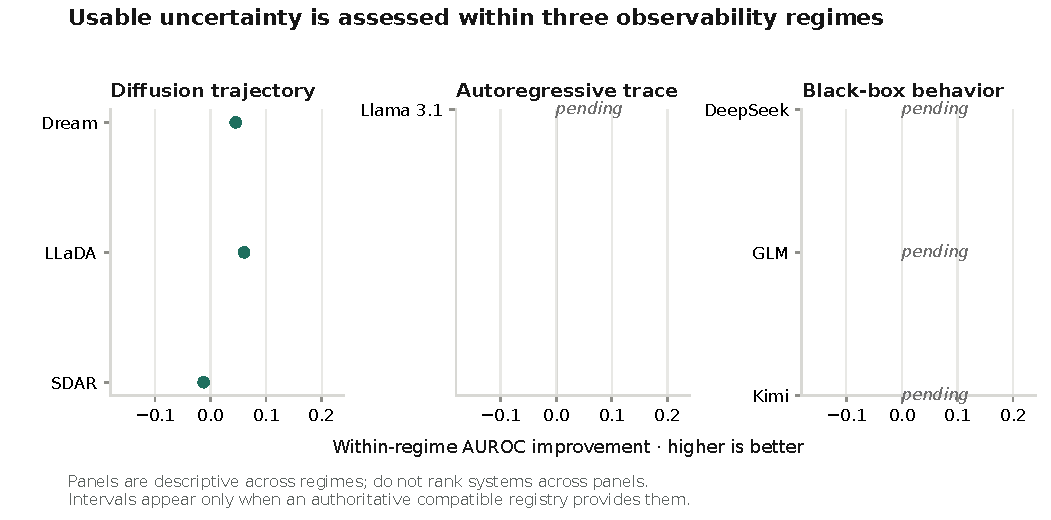
\includegraphics[width=0.98\textwidth]{figures/generated/cross_observability_synthesis.pdf}
\caption{Within-regime uncertainty improvement across three observability regimes. Panels deliberately separate diffusion-trajectory, autoregressive-trace, and black-box behavioral protocols; their horizontal positions are not a cross-regime statistical ranking. Points and intervals are shown only when a compatible authoritative registry supplies them. During execution, missing authoritative aggregates are labeled pending rather than estimated.}
\label{fig:cross-observability-synthesis}
\end{figure*}
}{}

\RQOneSummaryTable

\IfFileExists{figures/generated/primary_auroc_improvement_matrix.pdf}{
\begin{figure*}[t]
\centering
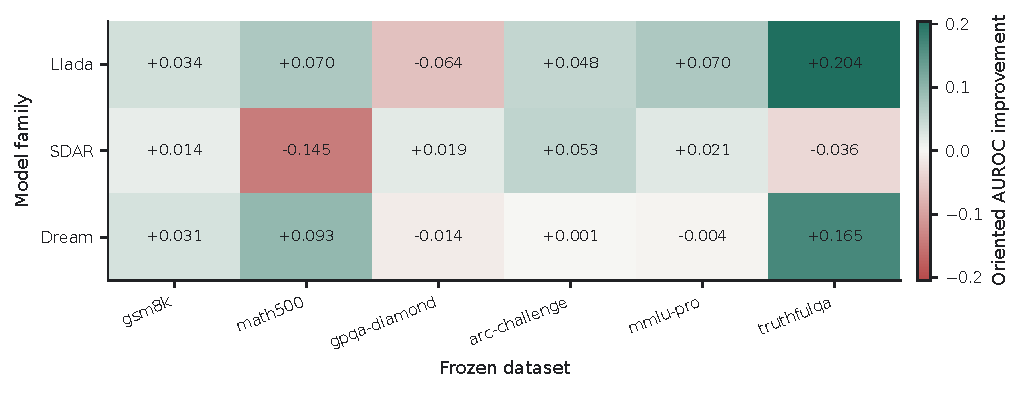
\includegraphics[width=0.96\textwidth]{figures/generated/primary_auroc_improvement_matrix.pdf}
\caption{Held-out AUROC improvement of \method over the matched decision-time entropy baseline for every frozen model--dataset cell. Positive values favor trajectory-aware uncertainty; the figure is rendered only from the complete provenance-bound 18-cell aggregate.}
\label{fig:primary-auroc-matrix}
\end{figure*}
}{}

\IfFileExists{figures/generated/rq1_feature_ablation.pdf}{
\begin{figure}[t]
\centering
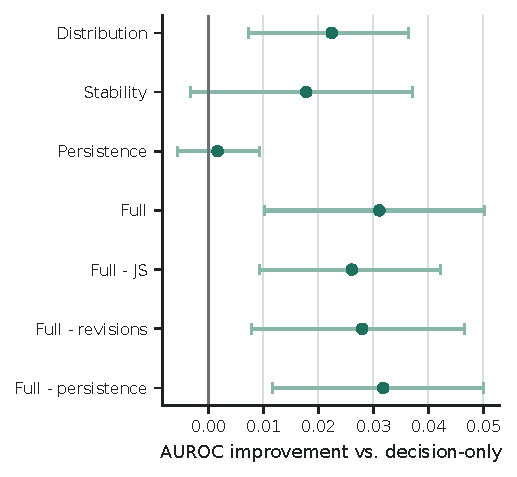
\includegraphics[width=0.96\columnwidth]{figures/generated/rq1_feature_ablation.pdf}
\caption{Frozen feature-family ablations relative to decision-only calibration. Points show equal-cell macro AUROC improvements and bars show paired 95\% confidence intervals.}
\label{fig:rq1-ablation}
\end{figure}
}{}

\begin{table}[t]
\centering
\small
\begin{tabular}{lccc}
\toprule
Method & AUROC $\uparrow$ & AUPRC $\uparrow$ & AURC $\downarrow$\\
\midrule
Repeated sampling & \RepeatedAUROC & \RepeatedAUPRC & \RepeatedAURC\\
\method (single trajectory) & \RepeatedTrajAUROC & \RepeatedTrajAUPRC & \RepeatedTrajAURC\\
\bottomrule
\end{tabular}
\caption{Expensive five-sample baseline on the pre-registered \RepeatedCellCount-cell ($3\times\RepeatedDatasetCount$) representative subset spanning GSM8K, MATH-500, GPQA-Diamond, and MMLU-Pro. The five auxiliary generations require \RepeatedAuxWallTime\ s/example on average (equal-cell macro; target generation excluded). MATH-500 votes use reference-free pairwise symbolic-equivalence clustering. ARC-Challenge and TruthfulQA remain in the complete 18-cell primary and adaptive analyses but are excluded from this secondary compute-intensive comparator before outcomes are observed.}
\label{tab:repeated}
\end{table}

\begin{table}[t]
\centering
\small
\begin{tabular}{lccc}
\toprule
Policy & Accuracy $\uparrow$ & Cost/base $\downarrow$ & $\Delta$ vs.\ random\\
\midrule
Base budget & \AdaptiveBaseAccuracy & \AdaptiveBaseCost & --\\
Fixed refined & \AdaptiveRefinedAccuracy & \AdaptiveRefinedCost & --\\
Random matched & \AdaptiveRandomAccuracy & \AdaptiveRandomCost & 0\\
\method adaptive & \AdaptiveAccuracy & \AdaptiveCost & \AdaptiveDeltaRandom\\
\bottomrule
\end{tabular}
\caption{Primary adaptive second-pass evaluation at the frozen 50\% selection cap, macro-averaged over all 18 cells. Cost is normalized to the complete base-generation budget; 25\% and 75\% caps are sensitivity analyses.}
\label{tab:adaptive}
\end{table}

\section{Analysis Plan}

We will first test whether trajectory information improves the nested decision-entropy baseline.
We then analyze calibration and risk--coverage behavior, feature-family ablations, budget sensitivity, and failure cases. The frozen ablations are aggregated over all 18 cells with the same paired class-stratified within-cell bootstrap and equal-cell macro-averaging, and are reported in Appendix~\ref{tab:feature-ablation}.
For FLARE, same-checkpoint AR/diffusion disagreement is treated as a diagnostic feature, never as ground truth.
Negative results do not trigger post-hoc feature redesign on final test labels.
RQ5 is analyzed only after its separately hashed prospective freeze. Its
behavioral calibrators are fit on calibration partitions and evaluated on the
corresponding held-out tests with the same equal-cell principle, paired
class-stratified bootstrap, and Holm correction. The confirmatory questions
concern black-box selective prediction, cross-family heterogeneity, and the
observability gap relative to the open-model regimes; positive, negative,
null, and heterogeneous outcomes are retained.

\section{Conclusion}

\ConclusionResultSentence\ 
\method treats iterative denoising as an observable uncertainty process rather than merely a decoding mechanism.
Prior work already demonstrates useful dLLM-specific uncertainty signals \citep{zhong2026dise,vazhentsev2026dllmuq}; our central empirical question is therefore deliberately incremental and falsifiable. If a carefully calibrated trajectory model cannot improve over the matched decision-time baseline on held-out examples and multiple model families, then the additional trajectory telemetry should not be claimed to provide predictive value beyond decision-time confidence under our protocol.
The accompanying protocol is designed so that this conclusion can be reached without outcome leakage or post-hoc test tuning.

\section*{Limitations}

\PaperStateLimitationsSentence\ 
The primary evaluation focuses on answer-level correctness for reasoning and QA tasks; it does not establish calibration for long-form factuality, safety, or human preference.
Trajectory instrumentation is model-runtime dependent and must be parity-validated.
Exact full-vocabulary JS drift adds memory and compute overhead, which is measured but may reduce throughput.
Post-hoc logistic calibration requires a representative calibration partition and can degrade under distribution shift.
Single-split benchmarks use internal holdouts, so their values are not directly comparable to standard full-benchmark leaderboard scores.
For compute-bounded reproducibility, GSM8K and the larger ARC-Challenge/MMLU-Pro
partitions use predeclared deterministic caps; consequently those reported
numbers are frozen-subset estimates rather than full-split leaderboard scores.
The repeated-sampling baseline has substantially higher inference cost. For MATH-500, its vote classes depend on the pinned symbolic-equivalence parser; parser failures or unsupported expressions can still merge or split equivalence classes imperfectly.
Finally, adaptive refinement is evaluated with two frozen budgets; richer dynamic schedules are left to future work.
The hosted RQ5 models are provider-managed systems: exact server-side weights,
kernels, and routing are not inspectable, and provider revisions can change
despite stable public identifiers. RQ5 therefore binds the requested and
returned identifiers, capture time, provider trace metadata, pricing snapshot,
and raw response. Its conclusions are about deployment-visible behavior under
that frozen request contract, not mechanistic equivalence to open models.

\section*{Ethical Considerations}

Better uncertainty estimates can support abstention and compute allocation, but they do not make model outputs inherently safe or correct.
A calibrated score is task- and distribution-dependent and should not be interpreted as a universal probability of truth.
We avoid using correctness labels during generation and record provenance needed to audit reported numbers.
No proprietary user data are required by the frozen benchmark suite.
Gated datasets are used according to their access conditions and are not redistributed.

\bibliographystyle{tmlr}
\bibliography{references}
\appendix
\section{Appendix Overview}

The appendix contains the complete pre-results experimental contract.
It is intentionally detailed so that model-specific implementation choices cannot be changed silently after test outcomes are observed.

\section{Trajectory Telemetry Contract}

\paragraph{Eligibility.}
At every observation, predictive statistics are pooled only over positions that are active for the current block and unresolved.
Prompt tokens, inactive future blocks, and committed tokens are excluded.

\paragraph{Observation time.}
Telemetry is captured after the model produces logits and before the sampler commits/remasks tokens.
This makes every uncertainty feature pre-decision with respect to that denoising step.

\paragraph{JS drift.}
Exact Jensen--Shannon drift is calculated from consecutive full-vocabulary distributions only when a position is unresolved in both observations.
One previous probability tensor is retained; no full trajectory of vocabulary distributions is stored.

\paragraph{Decision-time features.}
For each generated position, decision-time entropy, confidence, and margin use its last unresolved observation.
The baseline uses mean decision-time entropy.

\paragraph{Commitment time.}
If a token first appears committed at observation $k$, the decision is assigned to observation $k-1$.
A token still unresolved in the final pre-transfer observation is assigned the final active decision index.

\section{Frozen Feature Definitions}

\begin{table*}[t]
\centering
\small
\begin{tabular}{lll}
\toprule
Family & Feature & Definition\\
\midrule
Decision & decision\_entropy\_mean & mean normalized entropy immediately before each token commitment\\
Distribution & entropy\_mean & mean normalized entropy over active unresolved positions\\
Distribution & entropy\_p90 & 90th percentile of normalized entropy\\
Distribution & entropy\_slope & linear early-to-late trend of step-level entropy\\
Distribution & margin\_mean / margin\_min & top-1 minus top-2 probability margin\\
Stability & js\_mean / js\_p90 & consecutive-step normalized JS drift\\
Stability & js\_slope / late\_js\_mean & temporal and late-stage JS behavior\\
Stability & revision\_rate & top-1 proposal changes while unresolved\\
Stability & late\_revision\_rate & revision rate in the final quarter of observations\\
Persistence & mask\_auc & unresolved fraction integrated over active observations\\
Persistence & late\_mask\_fraction & unresolved fraction in late observations\\
Persistence & commitment\_time\_mean & normalized mean decision index\\
\bottomrule
\end{tabular}
\caption{Frozen primary feature dictionary.}
\end{table*}

\section{Calibration and Leakage Firewall}

Generation and scoring are two separate stages.
The raw JSONL record stores prompt hash, model/runtime revision, seed, generated text/token IDs, trajectory features, step summaries, and runtime metadata.
It must store neither the reference answer nor correctness.
The scorer later joins correctness only after verifying example identity and prompt hash.
Calibration and test IDs are disjoint and namespaced by dataset and immutable source split.

Feature selection, calibrator family, adaptive thresholds, and ablation definitions are frozen before final test evaluation.
The primary calibrator is standardized logistic regression.
Isotonic regression is a sensitivity analysis only when the calibration partition is large enough to support it.

\section{Model-Specific Parity Gates}

\subsection{LLaDA-MoE}

The instrumented sampler mirrors the public LLaDA low-confidence masked-diffusion loop.
A 20-prompt deterministic reference run without telemetry is compared against the instrumented run using exact generated token IDs.
Mask token ID, attention mask, transfer counts, model/tokenizer revision, and seed must match.
Primary results are blocked until exact parity passes.

\subsection{Dream}

Dream exposes a token-generation hook through its public diffusion interface.
We compare a native no-hook reference against the hook-enabled telemetry path on identical prompts, revision, seed, and decoding parameters.
Exact token-ID parity is required.

\subsection{SDAR}

SDAR operates blockwise.
Telemetry is captured from the active generated positions of each block before token transfer.
The adapter is compared against the pinned upstream block-diffusion runtime.
The aggregate feature semantics and block boundaries are recorded in run metadata.
Primary SDAR numbers are blocked until parity passes.

\subsection{FLARE / HybridDiffusion}

FLARE is used primarily for RQ4.
The native runtime trace is parsed externally rather than modifying the serving engine.
Top-$k$ trace entropy is treated only as a proxy and is never mislabeled as full-vocabulary entropy.
Same-checkpoint AR/diffusion disagreement is a diagnostic, not a correctness label.

\section{Dataset Split Policy}

\begin{table}[h]
\centering
\small
\begin{tabular}{lll}
\toprule
Dataset & Calibration & Test\\
\midrule
GSM8K & official train & official test\\
ARC-Challenge & official validation & official test\\
MMLU-Pro & official validation & official test\\
GPQA-Diamond & frozen internal holdout & frozen internal holdout\\
TruthfulQA & frozen internal holdout & frozen internal holdout\\
MATH-500 & frozen internal holdout & frozen internal holdout\\
\bottomrule
\end{tabular}
\caption{Planned split roles. Internal holdouts are created before model calls.}
\end{table}

All prepared example IDs are namespaced as
\texttt{dataset:source-split:item-id}
to prevent false overlap when official splits reuse integer row indices.

\section{Correctness Scoring}

Multiple-choice tasks use exact option-letter matching after extracting the explicit final answer.
GSM8K uses normalized numeric exact matching against the official answer field.
MATH-500 uses a pinned symbolic equivalence verifier; parser failures are conservatively counted as incorrect.
No LLM judge is used for the primary correctness labels.

\section{Primary Statistical Tests}

For each model--dataset cell, the primary nested comparison fits:
\begin{align}
\mathcal{M}_0 &: H^{\mathrm{dec}} \rightarrow P(\mathrm{error}),\\
\mathcal{M}_1 &: [H^{\mathrm{dec}}, z_{\mathrm{traj}}] \rightarrow P(\mathrm{error}).
\end{align}
Both are fit only on calibration examples and evaluated on the same test examples.
Paired class-stratified bootstrap resampling estimates confidence intervals for AUROC, AUPRC, and AURC differences.
AURC improvements are sign-normalized so positive always means the trajectory model is better.

\section{Feature-Family Ablations}

We freeze:
\begin{enumerate}
\item decision only;
\item decision + distribution features;
\item decision + stability features;
\item decision + persistence features;
\item full model;
\item full minus JS drift;
\item full minus revisions;
\item full minus persistence.
\end{enumerate}
Every ablation is calibrated on the same calibration partition and evaluated on the same test examples.

\section{Repeated-Sampling Baseline}

The expensive baseline draws five independent generations under a frozen sampling configuration.
Without consulting labels, final answers are canonicalized and summarized by:
variation ratio, normalized vote entropy, and unique-answer fraction.
These features are calibrated on the calibration partition.
All additional model calls are included in the compute report.
For MATH-500, repeated-sampling voting remains disabled until algebraic-equivalence clustering is available.

\section{Adaptive Compute}

At the base budget, trajectory features are calibrated into error probability.
To prevent optimistic threshold fitting, calibration-set policy scores are generated by stratified cross-fitting.
The threshold is chosen under a frozen maximum refinement fraction.
A final calibrator is then trained on all calibration examples and applied to test.
The threshold is not retuned on test.

We report policy accuracy, refinement fraction, mean compute, and paired bootstrap intervals for accuracy differences versus base, fully refined, and expected random refinement.

\section{Run Provenance}

Every reported number must be associated with:
\begin{itemize}
\item repository commit;
\item model and tokenizer repository plus immutable revision;
\item upstream runtime commit where applicable;
\item dataset repository/config/split and immutable revision/fingerprint;
\item prompt-template version;
\item seed and decoding configuration;
\item Python, PyTorch, Transformers, CUDA, and GPU information;
\item wall-clock time and peak allocated GPU memory;
\item raw and scored artifact SHA-256 hashes.
\end{itemize}

\section{Planned Result Tables}

The final appendix will contain:
per-model/per-dataset uncertainty metrics;
calibration sensitivity;
feature-family ablations;
denoising-budget sensitivity;
adaptive-compute results;
parity audits;
runtime/memory overhead;
and a failure taxonomy.
No cell is populated without a corresponding immutable result artifact.


\end{document}
